\documentclass[preprint,12pt]{elsarticle}
\usepackage{geometry}
%\geometry{letterpaper}                   % ... or a4paper or a5paper or ...
\usepackage{graphicx}
\usepackage{amssymb}
\usepackage{epstopdf}
%% Use the option review to obtain double line spacing
%% \documentclass[preprint,review,12pt]{elsarticle}

%% Use the options 1p,twocolumn; 3p; 3p,twocolumn; 5p; or 5p,twocolumn
%% for a journal layout:
%% \documentclass[final,1p,times]{elsarticle}
%% \documentclass[final,1p,times,twocolumn]{elsarticle}
%% \documentclass[final,3p,times]{elsarticle}
%% \documentclass[final,3p,times,twocolumn]{elsarticle}
%% \documentclass[final,5p,times]{elsarticle}
%% \documentclass[final,5p,times,twocolumn]{elsarticle}

%% if you use PostScript figures in your article
%% use the graphics package for simple commands
%% \usepackage{graphics}
%% or use the graphicx package for more complicated commands
%% \usepackage{graphicx}
%% or use the epsfig package if you prefer to use the old commands
%% \usepackage{epsfig}

%% The amssymb package provides various useful mathematical symbols
\usepackage{amssymb}
%% The amsthm package provides extended theorem environments
%% \usepackage{amsthm}

%% The lineno packages adds line numbers. Start line numbering with
%% \begin{linenumbers}, end it with \end{linenumbers}. Or switch it on
%% for the whole article with \linenumbers after \end{frontmatter}.
%% \usepackage{lineno}

%% natbib.sty is loaded by default. However, natbib options can be
%% provided with \biboptions{...} command. Following options are
%% valid:

%%   round  -  round parentheses are used (default)
%%   square -  square brackets are used   [option]
%%   curly  -  curly braces are used      {option}
%%   angle  -  angle brackets are used    <option>
%%   semicolon  -  multiple citations separated by semi-colon
%%   colon  - same as semicolon, an earlier confusion
%%   comma  -  separated by comma
%%   numbers-  selects numerical citations
%%   super  -  numerical citations as superscripts
%%   sort   -  sorts multiple citations according to order in ref. list
%%   sort&compress   -  like sort, but also compresses numerical citations
%%   compress - compresses without sorting
%%
%% \biboptions{comma,round}

% \biboptions{}


\journal{Journal of Systems and Software}

%%% OUR MACROS %%%
\newcommand{\COMMENT}[1]{ } 

\begin{document}

\begin{frontmatter}

%% Title, authors and addresses

%% use the tnoteref command within \title for footnotes;
%% use the tnotetext command for the associated footnote;
%% use the fnref command within \author or \address for footnotes;
%% use the fntext command for the associated footnote;
%% use the corref command within \author for corresponding author footnotes;
%% use the cortext command for the associated footnote;
%% use the ead command for the email address,
%% and the form \ead[url] for the home page:
%%
%% \title{Title\tnoteref{label1}}
%% \tnotetext[label1]{}
%% \author{Name\corref{cor1}\fnref{label2}}
%% \ead{email address}
%% \ead[url]{home page}
%% \fntext[label2]{}
%% \cortext[cor1]{}
%% \address{Address\fnref{label3}}
%% \fntext[label3]{}

\title{$\pi$SOD-M: A Methodology for Building Service-Oriented Applications in
the Presence of Non-Functional Properties}

%% use optional labels to link authors explicitly to addresses:
%% \author[label1,label2]{<author name>}
%% \address[label1]{<address>}
%% \address[label2]{<address>} 
 
\author[inst1]{Pl\'acido A. Souza Neto}
\author[inst2]{Genoveva Vargas-Solar}
\author[inst3]{Martin A. Musicante}
\author[inst4]{Valeria~de~Castro}
\author[inst3]{Umberto Souza da Costa}

\address[inst1]{Federal Technological Institute of Rio Grande do Norte -- Natal-RN,
Brazil}

\address[inst2]{Universit\'e de Grenoble -- Saint Martin d'H\`{e}res, France}

\address[inst3]{Federal University of Rio Grande do Norte -- Natal-RN,
Brazil}

\address[inst4]{Universidad Rey Juan Carlos -- M\'{o}stoles, Spain}

\begin{abstract}
This paper presents\ldots
\end{abstract}

\begin{keyword}
%% keywords here, in the form: keyword \sep keyword

%% MSC codes here, in the form: \MSC code \sep code
%% or \MSC[2008] code \sep code (2000 is the default)

\end{keyword}

\end{frontmatter}

%%
%% Start line numbering here if you want
%%
% \linenumbers

%% main text
%*********************************************************************************************************
\section{Introduction}
\label{sec:intro}
\[ \mathbb{Intro\ SAC} \]

Functional properties of a computer system are characterized by the effect produced by the system when given a defined input.
Functional properties are not the only crucial aspect in the software development process. 
Other properties need to be addressed to fit in the application with its context.
These other aspects are called Non-Functional Properties.

Non-Functional Requirements (NFRs) specify those properties that are not addressed by the functional  specification.
They are often called \textit{qualities} of the software system.
%They are also referred as ``constraints'', ``quality attributes'', ``quality goals'', ``quality of
%service requirements'' and ``non-behavioural requirements'' \cite{Stellman2005}.
Non-Functional Requirements may specify response time, security constraints or quality of the solution, among others.




Service-Oriented Computing~\cite{Papazoglou2007}, is a software development paradigm where pre-existing services are combined to produce more complex applications. 
%The selection of services is usually guided by the functional requirements of the application. 
%In this scenario, there exists the need to provide support for the specification of non-functional requirements, such as
%security, reliability, and efficiency. 
The development of service-based applications can benefit from the inclusion of NFRs to the software process from its early stages.
Failure to comply with this inclusion means that the final application is obtained from a partial specification, making the deployment a difficult task.
%Ideally, non-functional requirements
%would be considered along with all the stages of the software development. 
The adoption of non-functional specifications from the early states of development
can help the developer to produce applications that are capable of dealing with
their context.
Non-functional properties of service oriented applications have been
addressed in academic works and standards~\cite{ws-co,ws-tra,wsci}.
Different proposals~\cite{Babamir2010,AgarwalLS09,CholletL09,GutierrezRF10,XiaoCZBOLH08,JeongCL09,TsadimasNA12}
support non-functional requirements in the context of web service development. 

Most software development methods define software processes that use the notion of refinement.
Software process begins with the formulation of an abstract specification, which is successively refined to yield the implementation of the system.
Methods for the development of web service applications are no exception to this rule.
At least two levels of abstraction can be distinguished: a \textit{Business Level}, including the abstract specification, and a \textit{System Level}, including actual computer programs that implements the system.

In the case of web service applications we will distinguish two separate layers of the implementation.
The \textit{Composition Layer} is the upper layer of the implementation. 
It defines the workflow of the system, in terms of individual service calls.
The \textit{Service Layer} defines those services that are called by the composition.

\[ \mathbb{Original} \]
Service oriented computing is at the origin of an evolution in the field of software development. 
An important challenge of service oriented development is  to ensure the alignment between IT systems and the business logic.
%dealing thereby with the promise that IT systems can  evolve  according to the business needs. 
Thus, organizations are  seeking for mechanisms to deal with the gap between the systems developed and business needs \cite{bell}. The literature stresses the need for methodologies and techniques for service oriented analysis and design, claiming that they are the cornerstone  in the development of meaningful services' based applications \cite{5}.  In this context, some authors argue that the convergence of model-driven software development, service orientation and better techniques for documenting and improving business processes are the key to make real the idea of rapid, accurate development of software that serves, rather than dictates, software users' goals \cite{watson}. 

Service oriented development methodologies providing models, best practices, and reference architectures to build services' based applications mainly address  functional aspects \cite{1,2,decastro1,PapazoglouH06}.  Non-functional aspects concerning services' and application's "semantics", often expressed as requirements and constraints in general purpose methodologies, are not fully considered or they are added once the application has been implemented in order to ensure some level of reliability (e.g., data privacy, exception handling, atomicity, data persistence). This leads to services' based applications that are partially specified and that are thereby partially compliant with application requirements.

The objective of this work   is to model non-functional constraints and associate them to  services' based applications  early during the services' composition modeling phase. Therefore this paper presents $\pi$-SOD-M, a model-driven method  that extends the SOD-M  \cite{decastro1} for building reliable  services' based information systems (SIS). 
%SOD-M defines a process  starting with the  identification of business services through business modeling, and, by means of models' transformations it allows to obtain a services' composition model \cite{decastro1} and the executable code that implements it. 

Our work proposes to extend the SOD-M \cite{decastro1} method with  (i)  the notion of {\em A-Policy} \cite{Espinosa-Oviedo2011a} for representing non-functional constraints associated to services' based applications.  
%{\em A-policies} are used to express constraints which can be applied to all the services' composition  or to a particular service used for implementing it. They represent both systems' cross-cutting aspects (e.g., exception handling expressing what to do when a service is not available) and use constraints imposed by the services  (e.g., the fact that a service requires imposes an authentication protocol for executing a method). 
Our work  also (ii) defines the $\pi$-{\sc Pews}  meta-model \cite{Placido2010LTPD} providing guidelines for expressing the composition and the {\em A-policies}. Finally, our work (iii) defines model to model transformation rules for generating the $\pi$-{\sc Pews} model of a reliable services' composition starting from the extended services' composition model; and, model to text transformations for generating the corresponding implementation. As will be shown within our environment implementing these meta models and rules, one may represent both systems' cross-cutting aspects (e.g., exception handling for describing what to do when a service is not available, recovery, persistence aspects) and constraints associated to services, that must be respected for using them (e.g., the fact that a service requires an authentication protocol for executing a method). 

The remainder of the paper is organized as follows. Section \ref{sec:motivation} gives an overview of our approach. It describes a motivation example that integrates and synchronizes well-known social networks services namely Facebook, Twitter and, Spotify. Sections \ref{sec:piscm}, \ref{sec:pewsmetamodel}, and \ref{sec:mmrules} describe respectively the three key elements of our proposal, namelly the $\pi$-SCM and $\pi$-{\sc Pews} meta-models and the transformation rules that support the semi-automatic generation of reliable services' compositions.
%describes $\pi$-SOD-M method that enables the representation and association of {\em A-policies} to services' composition  thereby making them reliable. 
%
Section \ref{sec:implementation} describes implementation and validation issues.
Section \ref{sec:related} analyses related work concerning policy/contract based programming and, services' composition platforms. Section \ref{sec:conclusions} concludes the paper and discusses future work.



%*********************************************************************************************************


%*********************************************************************************************************
\section{Modeling reliable services' compositions with $\pi$-SOD-M}\label{sec:motivation}

%Consider for instance the following scenario. An organization wants to provide the services' based application "To Publish Music" that monitors the music a person is listening during some periods of time and sends the song title  to this person's Twitter and Facebook accounts. Thus, this social network user will have her status synchronized in  Twitter and Facebook (i.e., either the same title is published in both accounts or it is not updated) with the title of the music she is listening in Spotify.
%For developing this services' based application it is necessary to compose the following services  calling  their  exported methods:
%\begin{itemize}
%\item The music service   Spotify exports a method for obtaining information  %about the music a given user is listening:
%%\begin{itemize} \item {\sf\small get-Last-Song ( userid ): String} ; %%\end{itemize}
%\item Facebook and Twitter services export a method for  updating the status of a given user:
%\begin{itemize} 
%%\item{\sf\small get-Status ( usedid ): String ; 
%\item {\sf\small update-Status ( userid, new-status ): String}; 
%\end{itemize}
%\end{itemize}
%
%Figure \ref{fig:E3valuemodel} shows the E3 value model \cite{e3value} of
%the scenario. The E3 value model is a business model that represents a business case graphically as a set of value exchanges ($\nabla$$\triangle$) and value activities (rounded boxes) performed by business actors (squared boxes) and allows us to understand the environment in which the services' composition will be placed. 
%The model in Figure \ref{fig:E3valuemodel} shows Spotify and a private application (which is also a service) that directly interact with users for providing free services for listening and publishing information about music being listened by users. The private application interacts with Spotify for obtaining free information about the flow of music being listened by a user in return of a fee (i.e., premium subscription). Finally, the private application interacts with Facebook and Twitter for updating the user's status and thereby they share non material benefits (i.e., the fact that users subscribe to their networks and are active on them thanks to the private application).

%Figure \ref{fig:E3valuemodel} shows the BPMN model  \footnote{Details on BPMN (Business Process Management Notation) can be found in http://www.bpmn.org/} of the scenario. 
%The "To Publish Music" scenario 
%%(showed by doted line) 
%starts by contacting the music service Spotify for retrieving the user's  musical status (activity {\sf Get Song}). 
%Twitter and Facebook services are then contacted in parallel for updating the user's status with the corresponding song title (activities {\sf Update Twitter} and {\sf Update Facebook}).
%\begin{figure}
%\centering
%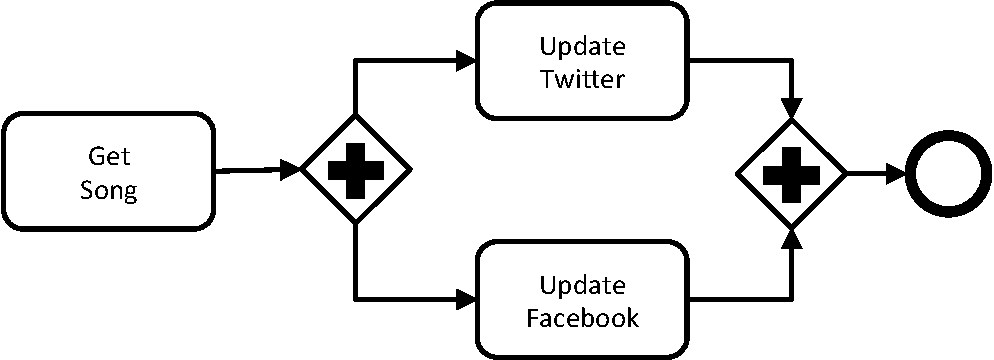
\includegraphics[width=0.55\textwidth]{figs/SC}
%\caption{BPMN model of the "To Publish Music" scenario}
%\label{fig:E3valuemodel}
%\end{figure}

Given a set of services with their exported methods known in advance or provided by a  service directory, building services' based applications can be  a simple task that implies expressing an application logic as a services' composition. The challenge being  ensuring the compliance between the specification and the resulting application. Software engineering methods (e.g., \cite{1,2,decastro1,PapazoglouH06}) today can help to ensure this compliance, particularly when information systems include several sometimes complex business processes calling Web services or legacy applications exported as services. 

%..--..--..--..--..--..--..--..--..--..--..--..--..--..--..--..--..--..--..--..--..--..--..--..--..--..--..--..--..--..--..--..--..--..--..--..--..--..--
\subsection{Modeling a services' based application}
%..--..--..--..--..--..--..--..--..--..--..--..--..--..--..--..--..--..--..--..--..--..--..--..--..--..--..--..--..--..--..--..--..--..--..--..--..--..--
 Figure \ref{fig:sodm} shows  SOD-M that defines a service oriented approach   providing  a set of guidelines to build services' based information systems (SIS) \cite{decastro1,decastro2}.  Therefore, SOD-M proposes to use services as first-class objects for the whole process of the SIS  development and it  follows a Model Driven Architecture (MDA) \cite{miller}  approach. Extending from the highest level of abstraction of the MDA, SOD-M provides  a conceptual structure to: first, capture the system requirements and specification in high-level abstraction models (computation independent models, CIMÕs); next,  starting from such models build platform independent models (PIMÕs) specifying the system details; next transform such models into platform specific models (PSMÕs) that bundles the specification of the system with the details of the targeted platform; and finally, serialize such model into the working-code that implements the system. 
\begin{figure} [htpb]
\centering
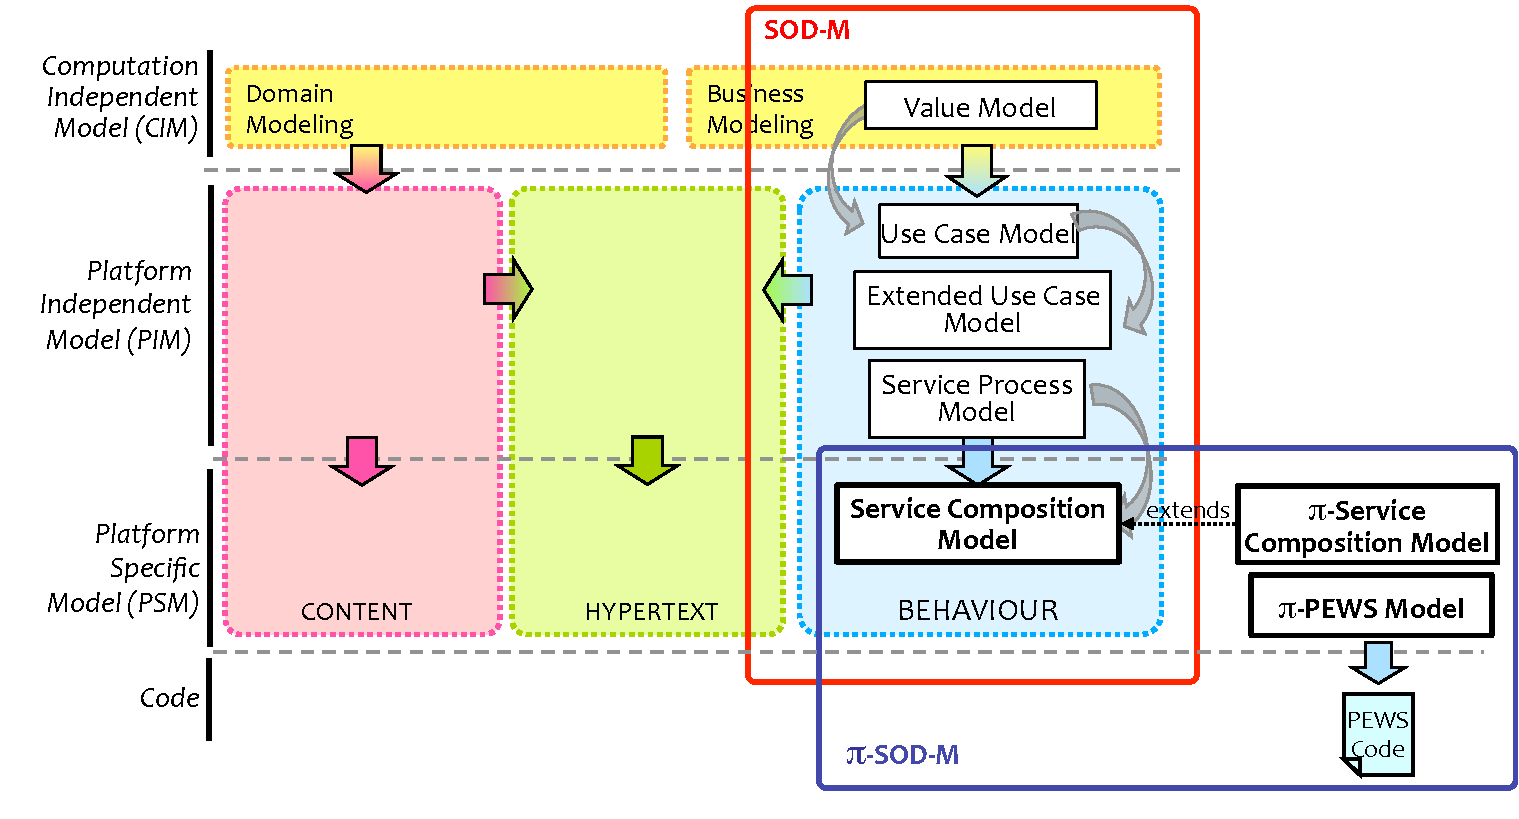
\includegraphics[width=0.65\textwidth]{figs/SODM}
\caption{SOD-M development process}
\label{fig:sodm}
\end{figure} 
As shown in Figure \ref{fig:sodm}, the SOD-M model-driven process begins by building the high-level computational independent models and enables specific models for a service platform to be obtained as a result  \cite{decastro1}. Referring to the "To Publish Music" application, using SOD-M the designer starts defining an E3value model \footnote{The E3 value model is a business model that represents a business case %graphically as a set of value exchanges ($\nabla$$\triangle$) and value activities (rounded boxes) performed by business actors (squared boxes) 
and allows  to understand the environment in which the services' composition will be placed \cite{e3value}.}  at the CIM level and then the corresponding models of the PIM are generated leading to a services' composition model (SCM).
%SOD-M proposes a set of models, :  i) the three different MDA abstraction levels: CIM, PIM and PSM; and ii) SOD-M views: business and information system views. 
%Model-Driven Engineering (MDE) \cite{schmidt} and particularly MDA \footnote{Model Driven Architecture (MDA)  is the particular model-driven proposal defined by the Object Management Group (OMG).} 
%provide
%is an evolving approach to software development that deals with the provision of 
%models, transformations between them and code generators to address software development. 
%One of the main advantages of model-driven approaches is the provision of 
%It also provides a conceptual structure where the models used by business managers and analysts can be traced towards more detailed models used by software developers.  

%Now, consider that besides the services' composition that represents the order in which the services are called for implementing the application "To Publish Music" it is necessary to model  other requirements that represent the (i) conditions imposed by services for being contacted, for example the fact the Facebook and Twitter require authentication protocol in order to call their methods for updating the wall; (ii) the conditions stemming from the business rules of the application logic, for example the fact that the walls in Facebook and Twitter must show the same song title and if this is not possible then none of them is updated. 

%..--..--..--..--..--..--..--..--..--..--..--..--..--..--..--..--..--..--..--..--..--..--..--..--..--..--..--..--..--..--..--..--..--..--..--..--..--..--
\subsection{Modeling non-functional constraints of services' based applications}
%..--..--..--..--..--..--..--..--..--..--..--..--..--..--..--..--..--..--..--..--..--..--..--..--..--..--..--..--..--..--..--..--..--..--..--..--..--..--
Adding non-functional requirements and services constraints in the services' composition is a complex task that implies programming  protocols for instance authentication protocols to call a service in our example, and atomicity (exception handling and recovery) for ensuring a true synchronization of the results produced by the service methods calls.
% song title disseminated in the walls of the user's Facebook and Twitter accounts. 

Service oriented computing promotes ease of information systems' construction thanks, for instance, to services' reuse. Yet, this is not applied to non-functional constraints as the ones described previously, because they do not follow in general the same service oriented principle and because they are often not fully considered in the specification process of existing services' oriented development methods. Rather, they   are either supposed to be ensured by the underlying execution platform, or they are programmed through ad-hoc protocols. Besides,  they are partially or rarely methodologically derived from the application specification, and they are added once the code has been implemented. In consequence, the resulting application does not fully preserve the compliance and reuse expectations provided by the service oriented computing methods.

%..--..--..--..--..--..--..--..--..--..--..--..--..--..--..--..--..--..--..--..--..--..--..--..--..--..--..--..--..--..--..--..--..--..--..--..--..--..--
%\subsection{$\pi$-SOD-M}
%..--..--..--..--..--..--..--..--..--..--..--..--..--..--..--..--..--..--..--..--..--..--..--..--..--..--..--..--..--..--..--..--..--..--..--..--..--..--

%
%Our proposal, called $\pi$-SOD-M, extends the services' composition model of the SOD-M method  with the notion of {\em A-Policy} \cite{Espinosa-Oviedo2011a} for representing services' composition constraints. 
%
Our work extends SOD-M for building applications by modeling the application logic and its associated non-functional constraints and thereby ensuring the generation of reliable services' composition. 
%This method is described in the following sections.
As a first step in our approach, and for the sake of simplicity we started modeling non-functional constraints at the PSM level. Thus, in this paper we  propose the $\pi$-SCM, the services' composition meta-model extended with {\em A-policies} for modeling non-functional constraints (highlighted in Figure  \ref{fig:sodm} and described in Section \ref{sec:piscm}).  $\pi$-SOD-M defines the $\pi$-{\sc Pews}  meta-model providing guidelines for expressing the services' composition and the {\em A-policies} (see Section \ref{sec:pewsmetamodel}), and also defines model to model transformation rules for generating  $\pi$-{\sc Pews} models starting from $\pi$-SCM models that will support executable code generation (see Section \ref{sec:mmrules}). Finally, our work defines model to text transformation rules for generating the program that implements both the services' composition and the associated {\em A-policies} and that is executed by an adapted engine (see Section \ref{sec:implementation}).


%*********************************************************************************************************

%*********************************************************************************************************
\section{$\pi$ services' composition meta-model}\label{sec:piscm}

The {\em A-policy} based services' composition meta-model (see  in Figure \ref{fig:servicecompositionmodel})
represents  a workflow needed to implement a services' composition, identifying those entities that collaborate in the business processes (called {\sc Business Collaborators} \footnote{We use {\sc capitals} for referring to meta-models' classes.}) and the {\sc Actions} that  they perform. This model is represented by means of a UML activity diagram. Thus, as shown in Figure \ref{fig:e-scomposition-metamodel}, the meta-model includes typical modeling elements of the activity diagram such as {\sc ActivityNodes}, {\sc InitialNodes} and {\sc FinalNodes}, {\sc DecisionNodes}, etc., along with new elements defined by SOD-M such as {\sc Business Collaborators}, {\sc ServiceActivity} and {\sc Action} (see the white  elements   in Figure \ref{fig:servicecompositionmodel}).

\begin{itemize}
\item A {\sc Business Collaborator} element represents those entities that collaborate in the business processes by performing some of the required actions. They are graphically presented as a partition in the activity diagram. A collaborator can be either internal or external to the system being modelled. When the collaborator of the business is external to the system, the attribute {\sf\small IsExternal} \footnote{We use the {\sf sans serif} font for referring to models' classes defined using a meta-model.} of the collaborator is set to true.

\item {\sc Action}, a kind of {\sc ExecutableNode}, are represented in the model as an activity. Each action identified in the model describes a fundamental behaviour unit which represents some type of transformation or processing in the system being modelled. There are two types of actions: i) a WebService (attribute Type is {\sf\small WS}); and ii) a simple operation that is not supported by a Web Service, called an {\sc ActivityOperation} (attribute Type is {\sc AOP}).
    
\item The {\sc ServiceActivity} element is a composed activity that  must be carried out as part of a business service and is composed of one or more executable nodes.
\end{itemize}

 \begin{figure}[htpb]
\centering
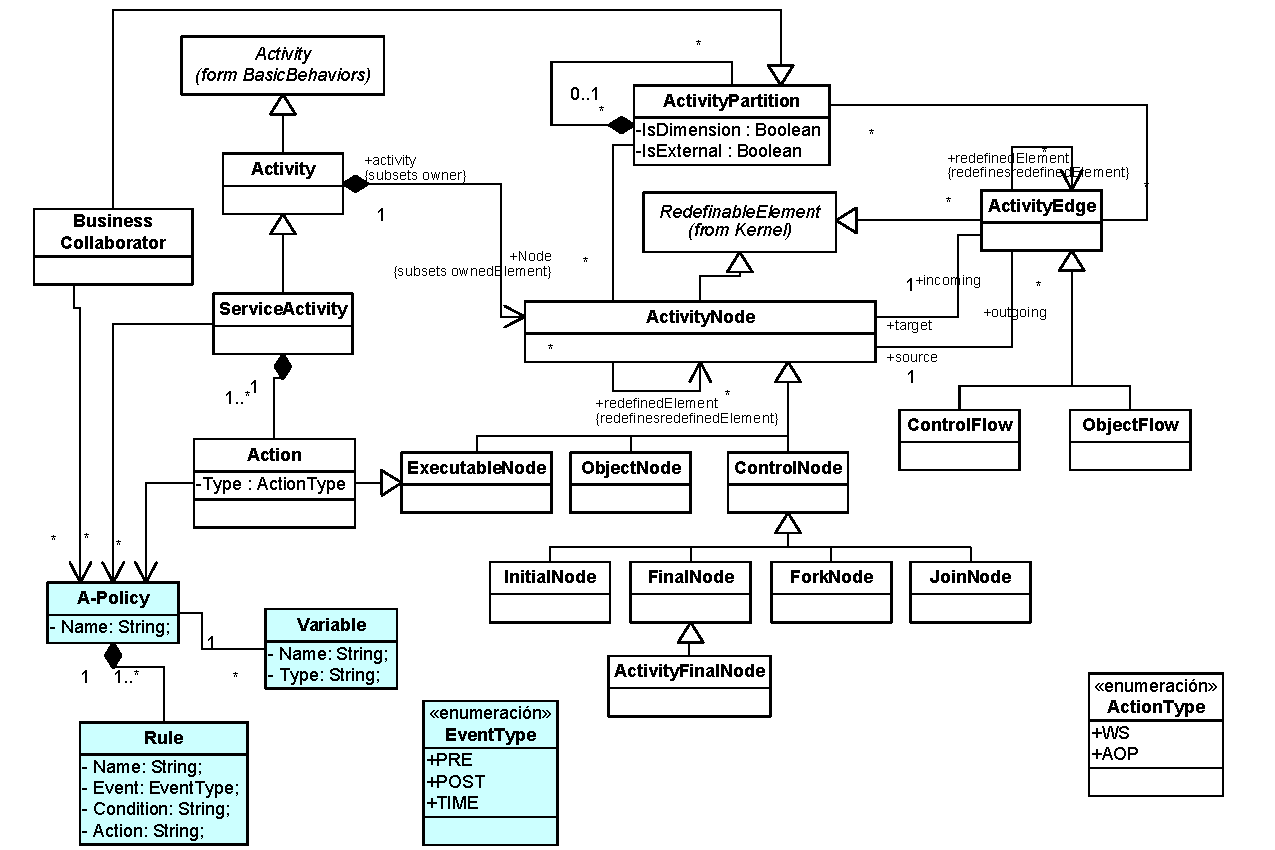
\includegraphics[width=0.80\textwidth]{figs/E-service-composition-metamodel}
\caption{{\em A-policy} based services' composition meta-model ($\pi$-SCM)}
\label{fig:e-scomposition-metamodel}
\end{figure}

To illustrate the use of the $\pi$-SCM meta-model we used it for defining the {\em A-policy} based composition model of the "To Publish Music" scenario (see
Figure \ref{fig:servicecompositionmodel}). There are three external business collaborators ({\em Spotify, Twitter} and {\em Facebook} \footnote{We use {\em italics} to refer to concrete values of the classes of a model that are derived from the classes of a meta-model.}). It also shows the business process  of the  "To Publish Music" application that consists of three service activities: {\em Listen Music}, {\em Public Music} and {\em Confirmation}. Note that  the action {\em Publish Music} of the application calls the actions of two service collaborators namely {\em Facebook} and {\em Twitter}.

Instead of programming different protocols within the application logic, we propose to include the modeling of non-functional constraints like transactional behaviour, security and adaptability  at the early stages of the services' composition engineering process. We model non-functional constraints of services' compositions using the notion of {\em A-policy} \cite{Espinosa-Oviedo2011a,CIC:eovszmc09c}, a kind of pattern for specifying {\em A-policy} types. In order to represent constraints associated to services compositions, we extended the SOD-M services' composition model with two concepts: {\sc Rule} and {\sc A-policy} (see blue elements in the $\pi$-SCM meta-model in Figure \ref{fig:e-scomposition-metamodel}).

The {\sc Rule} element represents an event - condition - action rule where the {\sc Event} part represents the moment in which a constraint  can be evaluated according to a condition represented by the {\sc Condition} part and the  action  to be executed for reinforcing  it represented by the {\sc Action} part. 
%An {\em A-policy}  describes  specific constraint types that can correspond to non-functional constraints like  transactional behaviour, security and adaptability. 
%An {\em A-policy}  defines a set of constraints over the execution states of the servicesÕ composition and defines strategies to enforce this property at the servicesÕ composition execution time.
An {\em A-policy} groups a set of rules. It describes global variables and operations that can be shared by the rules and that can be used for expressing their Event  and Condition parts. An {\em A-Policy} is associated to the elements {\sc BusinessCollaborator}, {\sc ServiceActivity} and, {\sc Action}  of the $\pi$-SCM meta-model (see Figure \ref{fig:e-scomposition-metamodel}) . 

\begin{figure}[htpb]
\centering
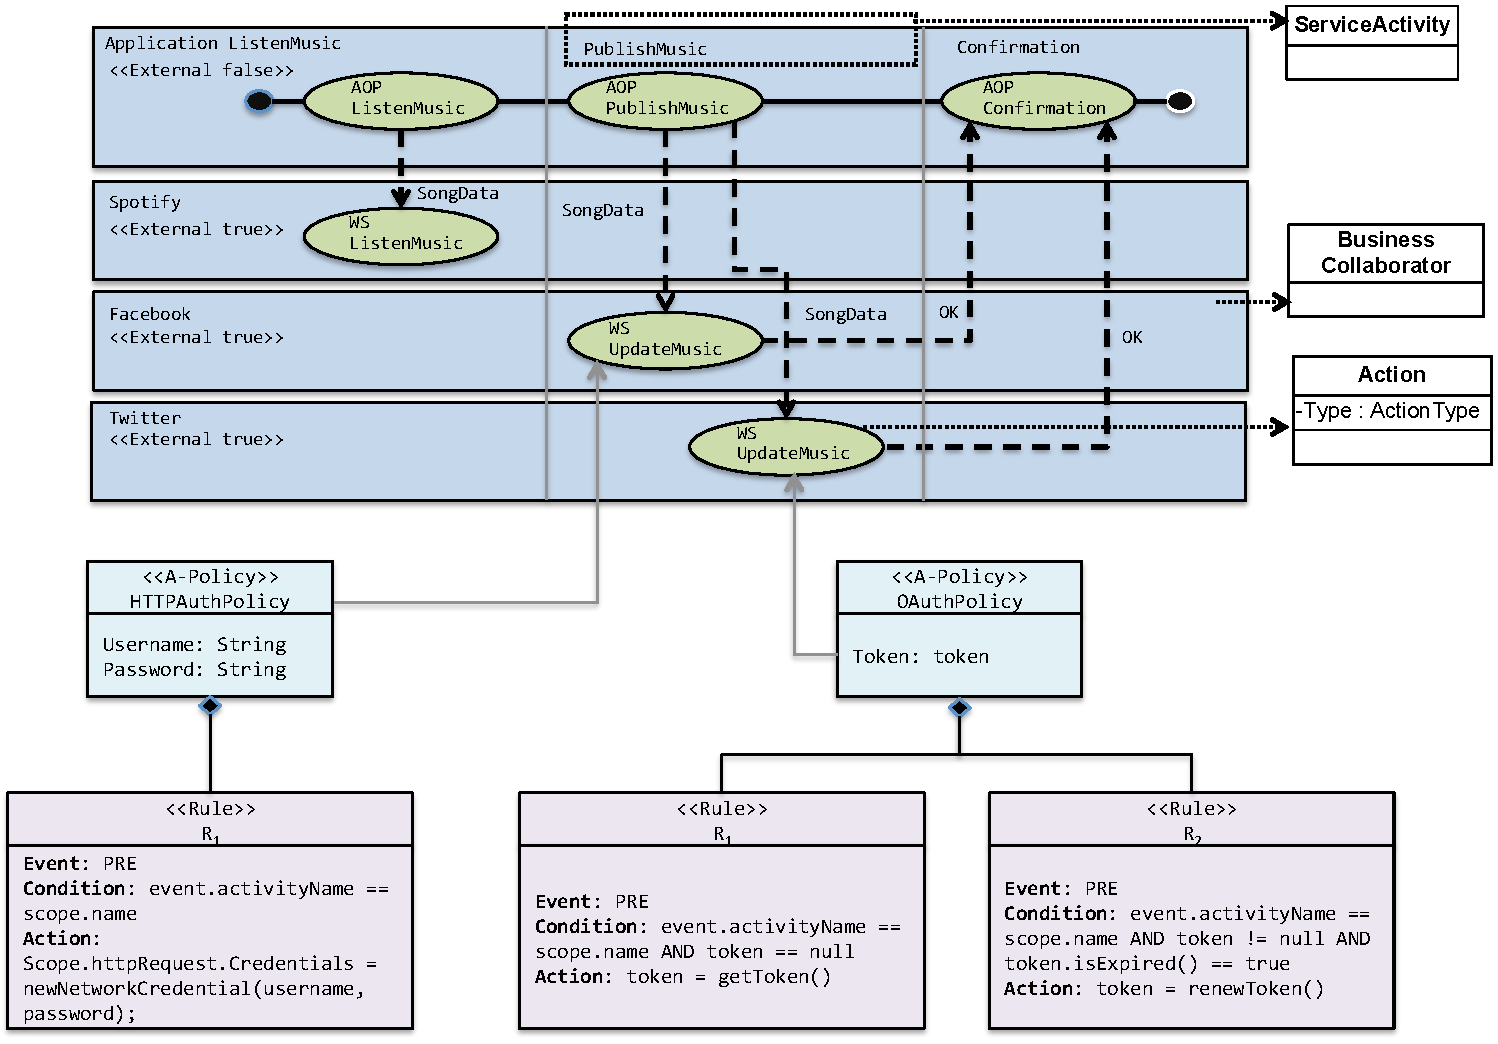
\includegraphics[width=0.70\textwidth]{figs/e-composition-model}
\caption{Services' composition model for the business service "To publish music"}
\label{fig:servicecompositionmodel}
\end{figure}

Given that {\em Facebook} and {\em Twitter} services require authentication protocols in order to execute methods that will read and update the users' space. A call to such services must be part of the authentication protocol required by these services.
In the example we  associate two authentication policies, one for the open authentication protocol, represented by the class {\sf\small Twitter OAuthPolicy} that will be associated to the activity  {\sf\small UpdateTwitter} (see Figure \ref{fig:servicecompositionmodel}). In the same way, the  class {\sf\small Facebook HTTPAuthPolicy}, for the http authentication protocol will be associated to the activity {\sf\small UpdateFacebook}.
 {\sf\small OAuth}  implements the open authentication protocol.
As shown in Figure \ref{fig:servicecompositionmodel}, the {\em A-policy} has a variable {\sf\small Token} that will be used to store the authentication token provided by the service. This variable type is imported through the library {\sf\small OAuth.Token}. The {\em A-policy}  defines two rules, both can be triggered by events of type {\sf\small ActivityPrepared}: (i) if no token has been associated to the variable {\sf\small token}, stated in by the condition of rule {\sf\small R$_1$}, then a token is obtained (action part of {\sf\small R$_1$}); (ii) if the token has expired, stated in the condition of rule {\sf\small R$_2$}, then it is renewed (action part of {\sf\small R$_2$}). Note that the code in the actions profits from the imported  {\sf\small OAuth.Token} for transparently obtaining or renewing a token from a third party.

{\sf\small HTTP-Auth} implements the HTTP-Auth protocol.  As shown in Figure  \ref{fig:servicecompositionmodel}, the {\em A-policy} imports an http protocol library and it has two variables {\sf\small username} and {\sf\small password}.  The event of type {\sf\small ActivityPrepared} is the triggering event of the rule {\sf\small R$_1$}. On the notification of an event of that type, a credential is obtained using the username and password values. The object storing the credential is associated to the scope, i.e., the activity that will then use it for executing the method call.

Thanks to rules and policies  it is possible to model and associate non-functional properties to services' compositions  and then generate the code. For example, the atomic integration of information retrieved from different social network services, automatic generation of an integrated view of the operations executed in different social networks or for providing security in the communication channel when the payment service is called.

Back to the  definition process of a SIS, once the {\em A-policy} based services' composition model has been defined, then it can be transformed into a model (i.e., $\pi$-PEWS model) that can support then executable code generation. The following Section describes the $\pi$-PEWS  meta-model that supports this representation. 


%..--..--..--..--..--..--..--..--..--..--..--..--..--..--..--..--..--..--..--..--..--..--..--..--..--..--..--..--..--..--..--..--..--..--..--..--..--..--
\section{$\pi$-{\sc Pews}  meta-model}\label{sec:pewsmetamodel}
%..--..--..--..--..--..--..--..--..--..--..--..--..--..--..--..--..--..--..--..--..--..--..--..--..--..--..--..--..--..--..--..--..--..--..--..--..--..--
The idea of the $\pi$-{\sc Pews} meta-model is based on the services' composition approach provided by the language PEWS\cite{BaAM06,Placido2010LTPD} (\textit{Path Expressions for Web Services}), a programming language that lets the service designer  combine the methods or subprograms that
implement each operation of a service, in order to achieve the desired application logic. Figure \ref{fig:metamodel} presents the $\pi$-{\sc Pews} meta-model
consisting of  classes representing:
\begin{itemize}
\item A services' composition: {\sc Namespace} representing the interface exported by a service, {\sc Operation} that represents a call to a service method, {\sc CompositeOperation}, and  {\sc Operator} for representing a services' composition and {\sc Path} representing a services' composition.
A {\sc Path} can be an {\sc Operation} or a {\sc Compound Operation}
denoted by an identifier. A {\sc Compound Operation} is defined using an  {\sc Operator}  that can be represent  sequential ($\ . \ $) and parallel ($\ \| \ $) composition of services,
 choice ($\ + \ $) among services,
the sequential ($*$) and parallel ($\{\dots\}$) repetition of an operation or the conditional execution of an operation ($[C]S$).

\item {\em A-Policies} that can be associated to a services' composition:  {\sc A-Policy}, {\sc Rule}, {\sc Event}, {\sc Condition}, {\sc Action}, {\sc State}, and {\sc Scope}.
\end{itemize}
%
\begin{figure}
\centering
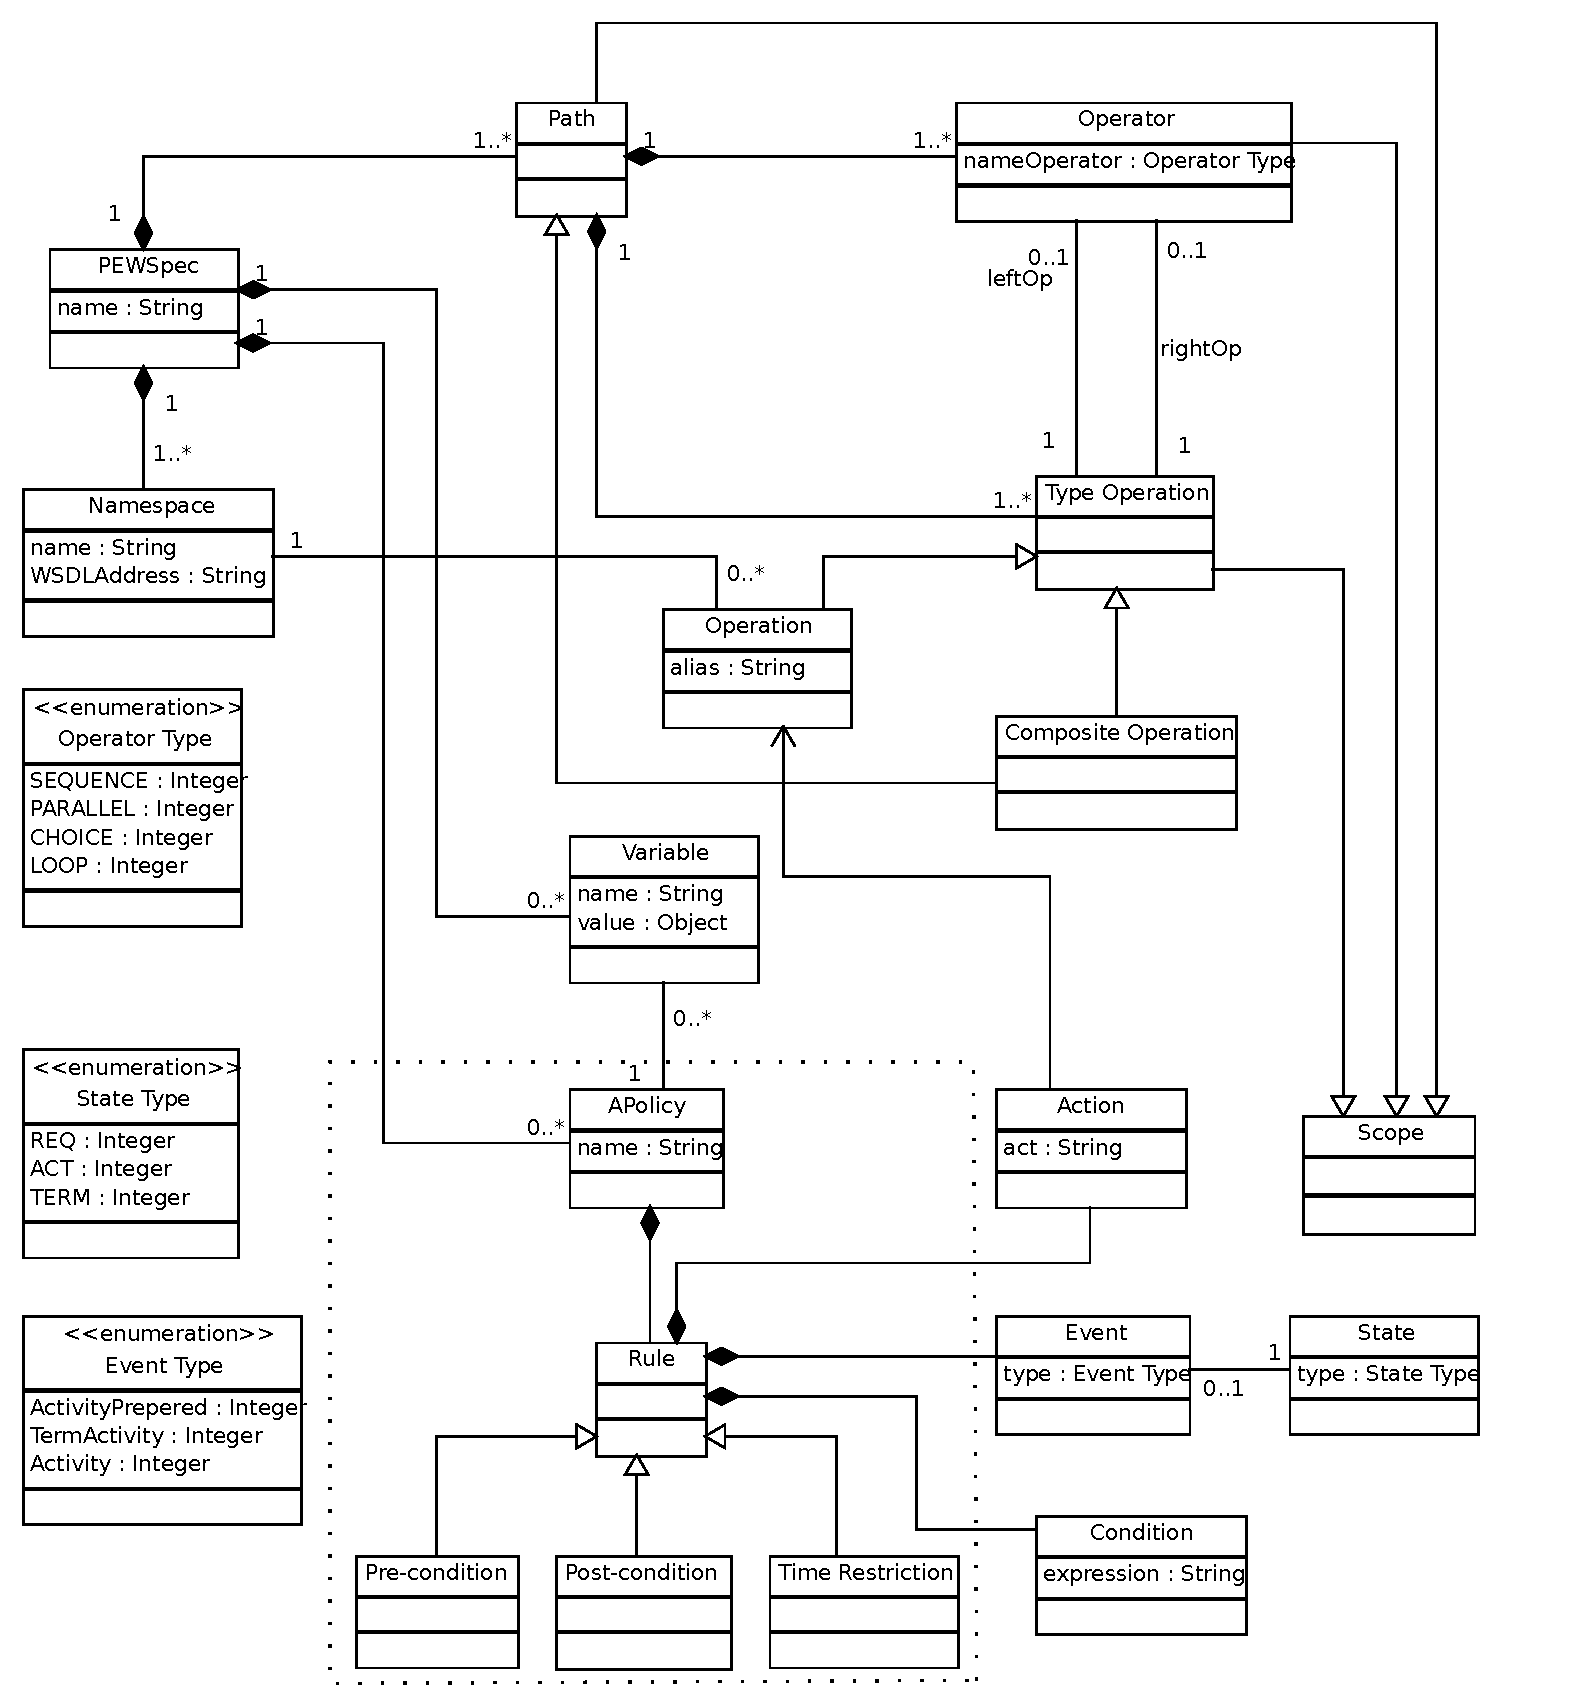
\includegraphics[width=0.80\textwidth]{figs/PEWSMetamodel}
\caption{$\pi$-{\sc Pews} Metamodel}
\label{fig:metamodel}
\end{figure}

As shown in the diagram an {\sc A-Policy} is applied to a {\sc Scope} that can be either an {\sc Operation} (e.g., an authentication protocol associated to a method exported by a service),  an {\sc Operator} (e.g., a temporal constraint associated to a sequence of operators, the authorized delay between reading a song title in Spotify and updating the walls must be less then 30 seconds), and a {\sc Path} (e.g., executing the walls' update under a strict atomicity protocol -- all or noting).  It groups a set of ECA rules, each rule having a classic semantics, i.e, {\em when an event of type E occurs if  condition C is verified then execute the action A}.  Thus, an {\em A-policy} represents a set of reactions to be possibly executed if one or several triggering events of its rules are notified.
\begin{itemize}
\item The class {\sc Scope} represents any element of a services' composition (i.e., operation, operator, path).
\item The class {\sc A-Policy} represents a recovery strategy implemented by ECA rules of the form {\sc Event} - {\sc Condition} - {\sc Action}. A {\em A-policy} has variables that represent the view of the execution state of its associated scope, that is required for executing the rules. The value of a variable is represented using the type {\sc Variable}. The class {\sc A-Policy} is specialized for defining specific constraints, for instance authentication {\em A-policies}.
\end{itemize}

%An authentication {\em A-policy} represents the situation where an invocation in
%an activity occurs until its sender and/or its recipient have been
%identified. Typically, authentication A-Policies ensure that the invocation of the activity will be done within an authentication protocol.
%

Given a $\pi$-SCM model of a specific services' based application (expressed according to the $\pi$-SCM meta-model), it is possible to generate its corresponding $\pi$-{\sc Pews} model thanks to transformation rules. The following Section describes the transformation rules between the $\pi$-SCM and $\pi$-{\sc Pews} meta-models of our method.

%..--..--..--..--..--..--..--..--..--..--..--..--..--..--..--..--..--..--..--..--..--..--..--..--..--..--..--..--..--..--..--..--..--..--..--..--..--..--
\section{Transformation rules}\label{sec:mmrules}
%..--..--..--..--..--..--..--..--..--..--..--..--..--..--..--..--..--..--..--..--..--..--..--..--..--..--..--..--..--..--..--..--..--..--..--..--..--..--

Figure \ref{fig:transformations} shows the transformation principle between the elements of the $\pi$-SCM meta-model used for representing the services' composition into the elements of the $\pi$-{\sc Pews} meta-model. There are two groups of rules: those that transform services' composition elements of the $\pi$-SCM to $\pi$-{\sc Pews} meta-models elements; and those that transform rules grouped by policies into {\em A-policy} types.

% _ . _ . _ . _ . _ . _ . _ . _ . _ . _ . _ . _ . _ . _ . _ . _ . _ . _ .
%\noindent

%{\bf\em 
\subsection{Transformation of the services' composition elements of the $\pi$-SCM to the $\pi$-{\sc Pews} elements}
% _ . _ . _ . _ . _ . _ . _ . _ . _ . _ . _ . _ . _ . _ . _ . _ . _ . _ .
A named action of the $\pi$-SCM represented by  {\sc\em Action} and {\sc\em Action:name} is transformed to a  named class {\sc Operation} with a corresponding attribute name {\sc Operation:name}. A  named service activity represented by the elements {\sc\em ServiceActivity}  and  {\sc\em ServiceActivity:name} of the $\pi$-SCM, are  transformed into a named operation of the $\pi$-{\sc Pews} represented by the elements  {\sc CompositeOperation} and {\sc CompositeOperation:name}. When more than one action is called, according to the following  composition patterns expressed using the operators {\sc\em merge, decision, fork and join} in the $\pi$-SCM the corresponding transformations, according to the PEWS operators presented above, are (see details in Figure \ref{fig:transformations}):
\begin{itemize}
\item   $op_1 . op_2$ if no {\sc\em ControlNode} is specified
\item ($op_1 \parallel op_2) . op_3$ if control nodes of type {\sc\em fork, join} are combined
 \item ($op_1 + op_2) . op_3$ if control nodes of type {\sc\em decision, merge} are combined
\end{itemize}

In the scenario "To Publish Music" the service activity {\sf PublishMusic} of the $\pi$-SC model specifies  calls to two {\sf Activitie}s of type {\em UpdateMusic}, respectively concerning the {\sf Business Service}s {\em Facebook} and {\em Twitter}. Given that no {\sf ConstrolNode} is specified by the $\pi$-SC model, the corresponding transformation is the expression that defines a {\sf Composite Operation} named {\em PublishSong} of the $\pi$-{\sc Pews} model of the form ({\sf PublishFacebook} $\parallel$ {\sf PublishTwitter}).
\begin{figure}
\centering{
%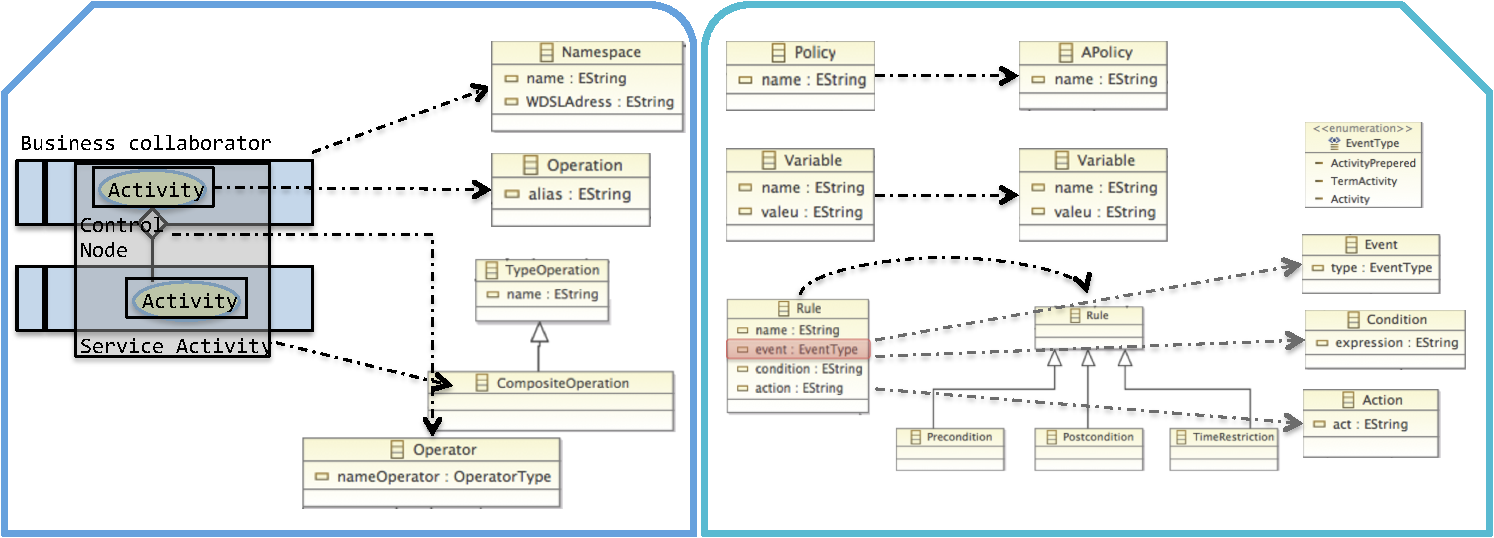
\includegraphics[width=0.80\textwidth]{figs/PI-SC-PI-P}}
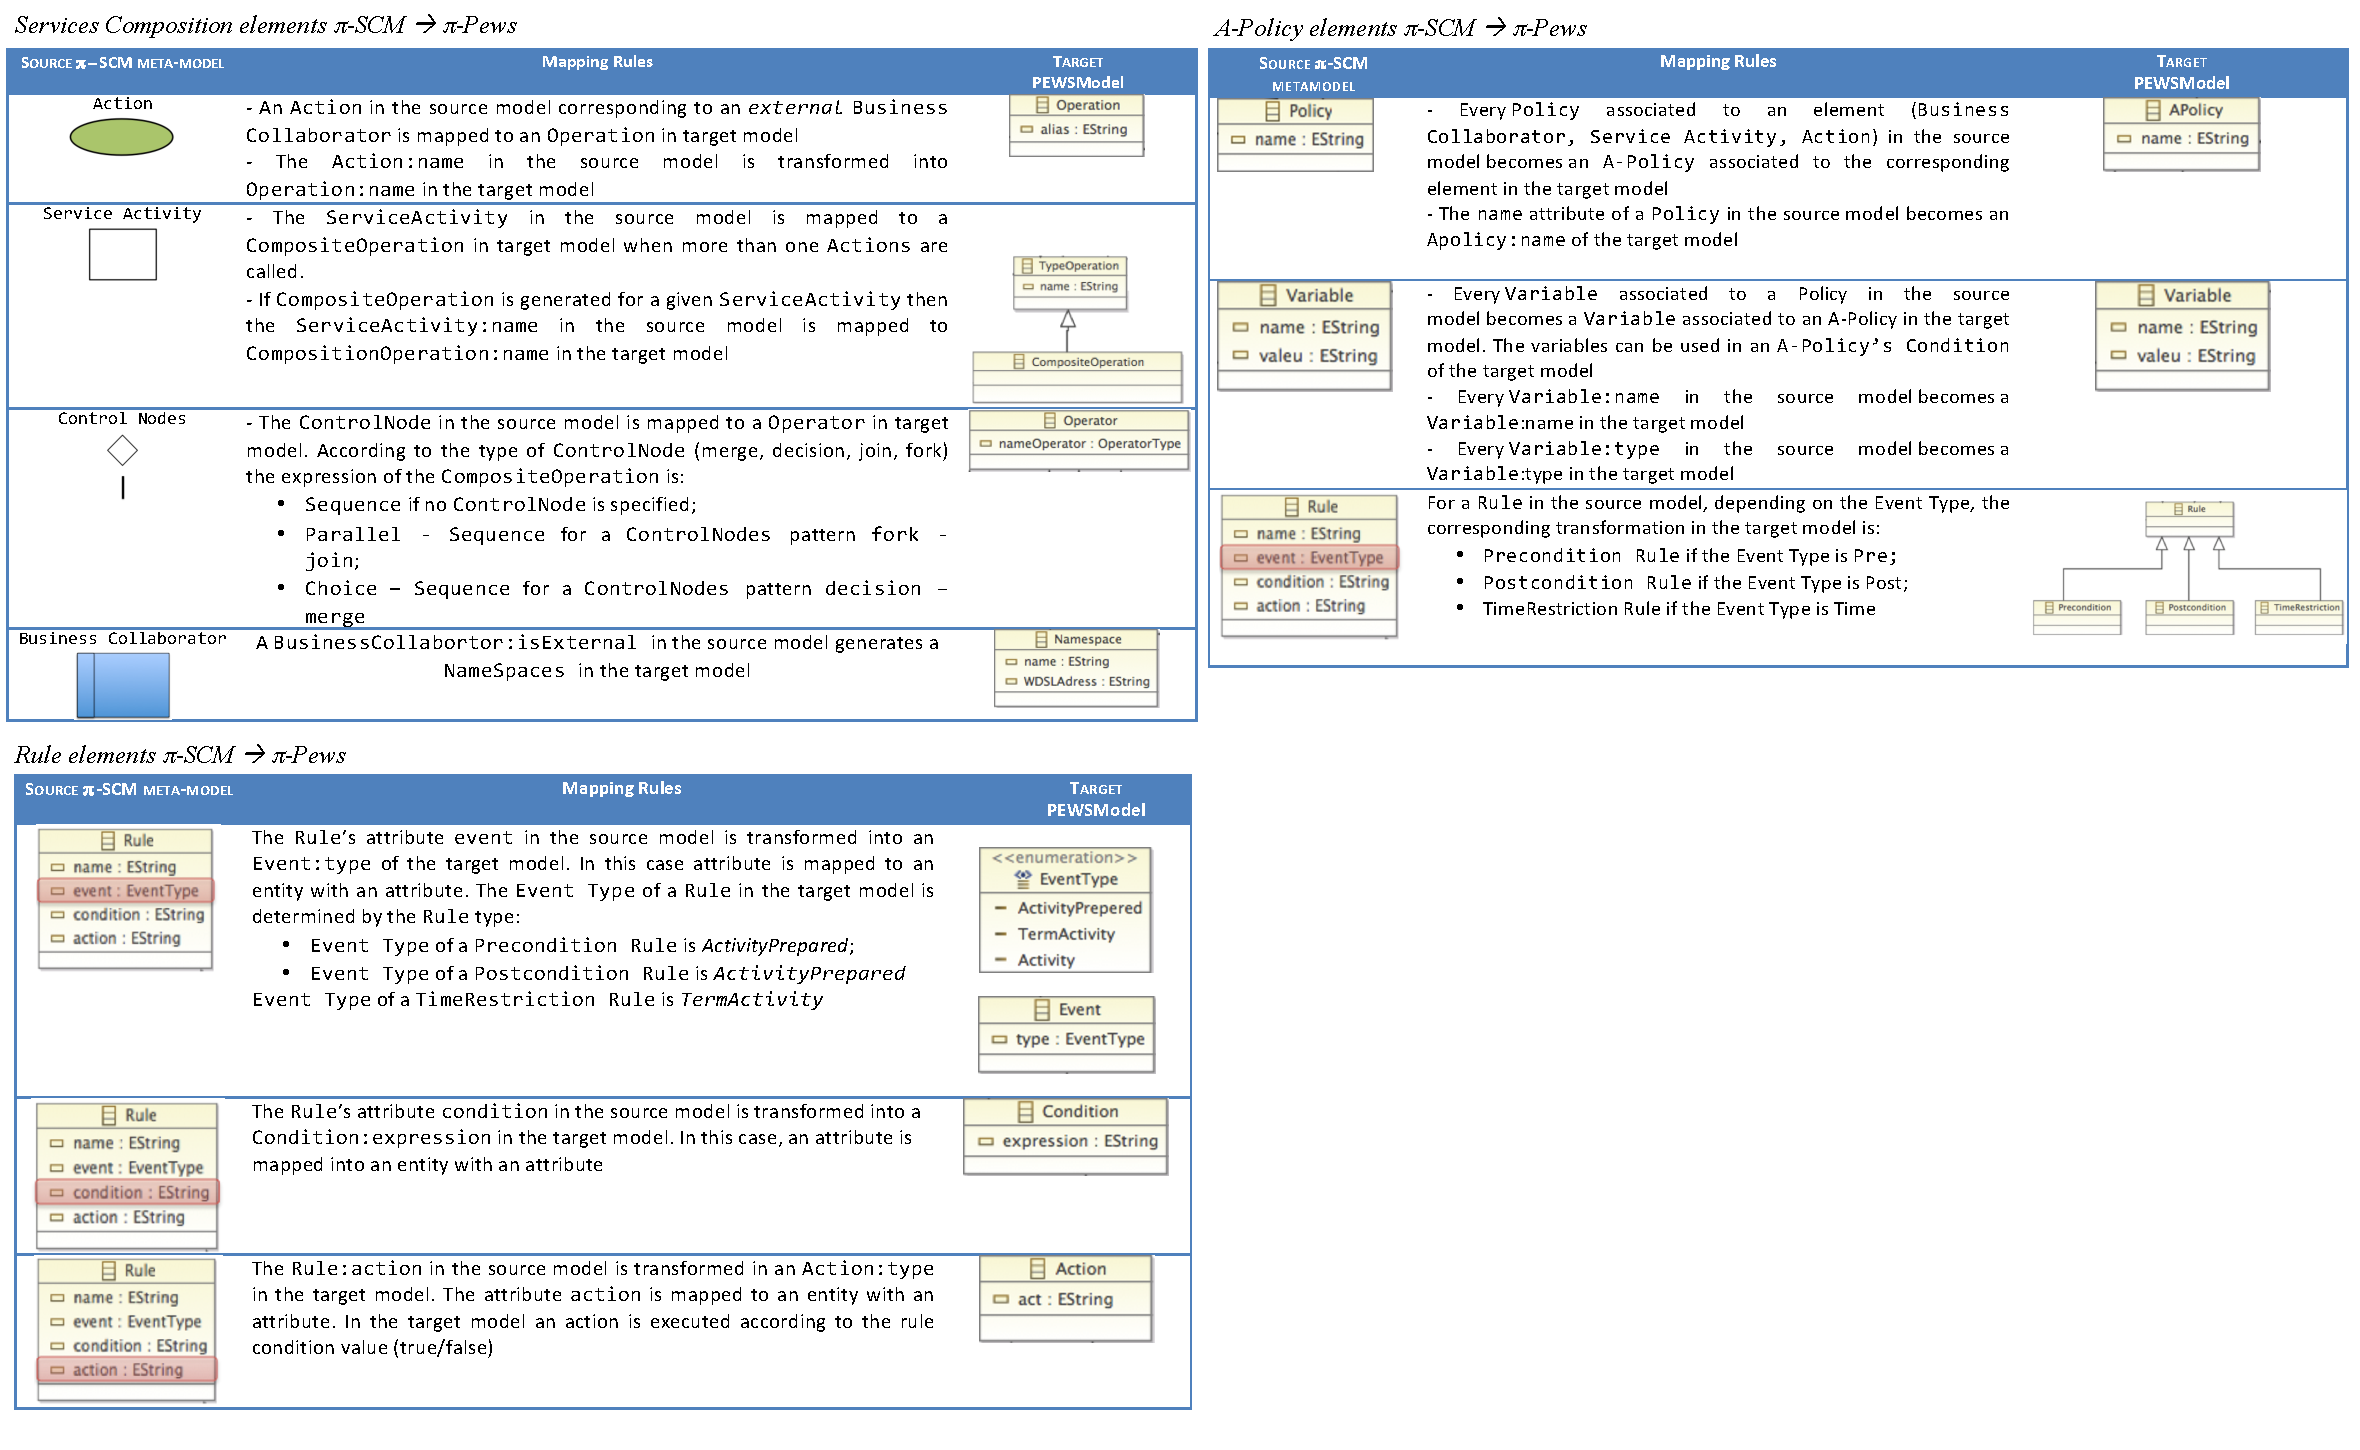
\includegraphics[width=0.96\textwidth]{figs/Mapping-1}}
\caption{ $\pi$-SCM to $\pi$-{\sc Pews} transformation}
\label{fig:transformations}
\end{figure}

% _ . _ . _ . _ . _ . _ . _ . _ . _ . _ . _ . _ . _ . _ . _ . _ . _ . _ .
%\noindent

%{\bf\em 
\subsection{Transformation of rules grouped by A-policies   in the $\pi$-SCM to A-Policies of  $\pi$-{\sc Pews}}
% _ . _ . _ . _ . _ . _ . _ . _ . _ . _ . _ . _ . _ . _ . _ . _ . _ . _ .
The {\em A-policies} defined for the elements of the $\pi$-SCM are transformed into {\sc A-Policy} classes, named according to the names expressed in the source model. The transformation of the rules expressed in the $\pi$-SCM is guided by the event types associated to these rules.   The variables associated to an {\em A-policy} expressed in the $\pi$-SCM as {\sc\em $<$Variable:name, Variable:type$>$} are transformed into elements of type {\sc Variable} with attributes {\sc name} and {\sc type} directly specified from the elements {\sc\em  Variable:name} and {\sc\em Variable:type} of the $\pi$-SCM model.

As shown in Figure \ref{fig:transformations}, for an event of type {\sc\em Pre} the corresponding transformed rule is of type {\sc Precondition}; for an event of type {\sc\em Post} the corresponding transformed rule is of type {\sc Postcondition}; finally, for an event of type {\sc\em TimeRestriction} the corresponding transformed rule is of type {\sc Time}. 
The condition expression of a rule in the $\pi$-SCM ({\sc\em Rule:condition}) is transformed into a class {\sc\em Condition:expression} where the attributes of the expression are transformed into elements of type {\sc Attribute}.

%The attribute event of a rule  ({\sc\em Rule:event}) in the $\pi$-SCM is transformed into an {\sc Event Type} according to the rule type. 

%As shown in Figure \ref{fig:transformations}, the event type for a rule of type (i) {\sc Precondition} is {\sc ActivityPrepared}; (ii) {\sc Postcondition} is {\sc TermActivity}; (iii) {\sc TimeRestriction} is {\sc Temporal}. The {\sc\em Rule:Action} of a rule in the $\pi$-SCM is transformed into an {\sc Action:type}.

%
%Figure \ref{fig:p-scim} shows the  $\pi$-{\sc Pews} model for our example.
In the scenario "To Publish Music" the {\sf Policies} {\em OAuthPolicy} and {\em HTTPAuthPolicy} of the $\pi$-SCM model are transformed into {\em A-policies} of type {\sf Precondition} of the $\pi$-{\sc Pews} model of the scenario. Thus in both cases the events are of type {\sf ActivityPrepared}. These policies, as stated in the $\pi$-SCM model, are associated to {\sf Activities}. In the corresponding transformation they are associated to {\sf Operation}s {\em PublishFacebook} and {\em PublishTwitter}.
%\begin{figure}[htpb]
%\centering{
%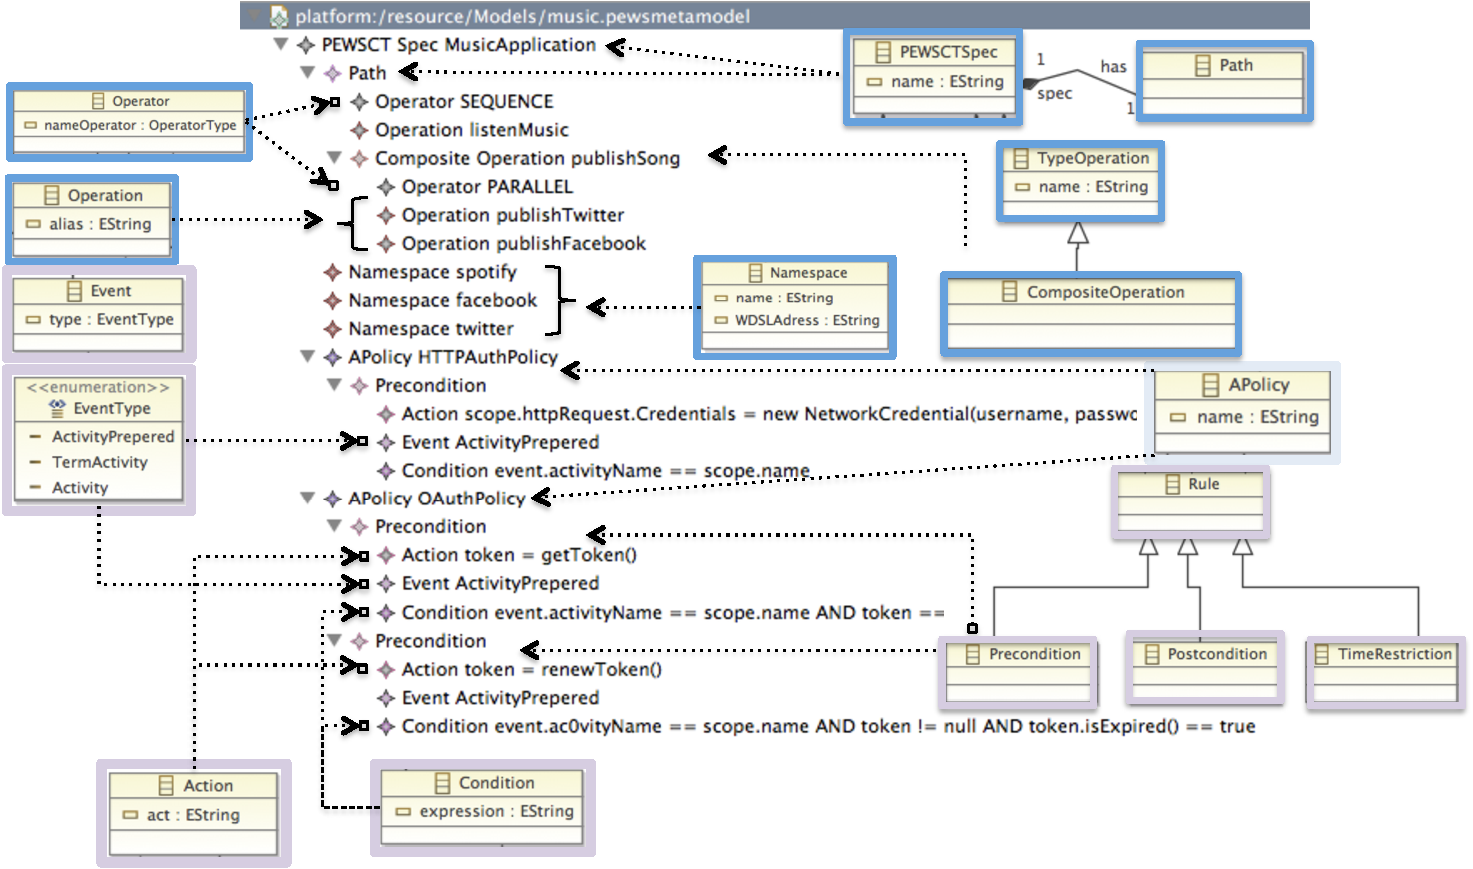
\includegraphics[width=0.78\textwidth]{figs/modeloPEWS}}
%\caption{$\pi$-{\sc Pews} generated model fo the "To Publish Music" application}
%\label{fig:p-scim}
%\end{figure}

%Figure \ref{fig:pewsexpression} shows the correspondence between the model and the statements that implement it, with a schematic representation of the business process.
%\begin{figure}
%\centering{
%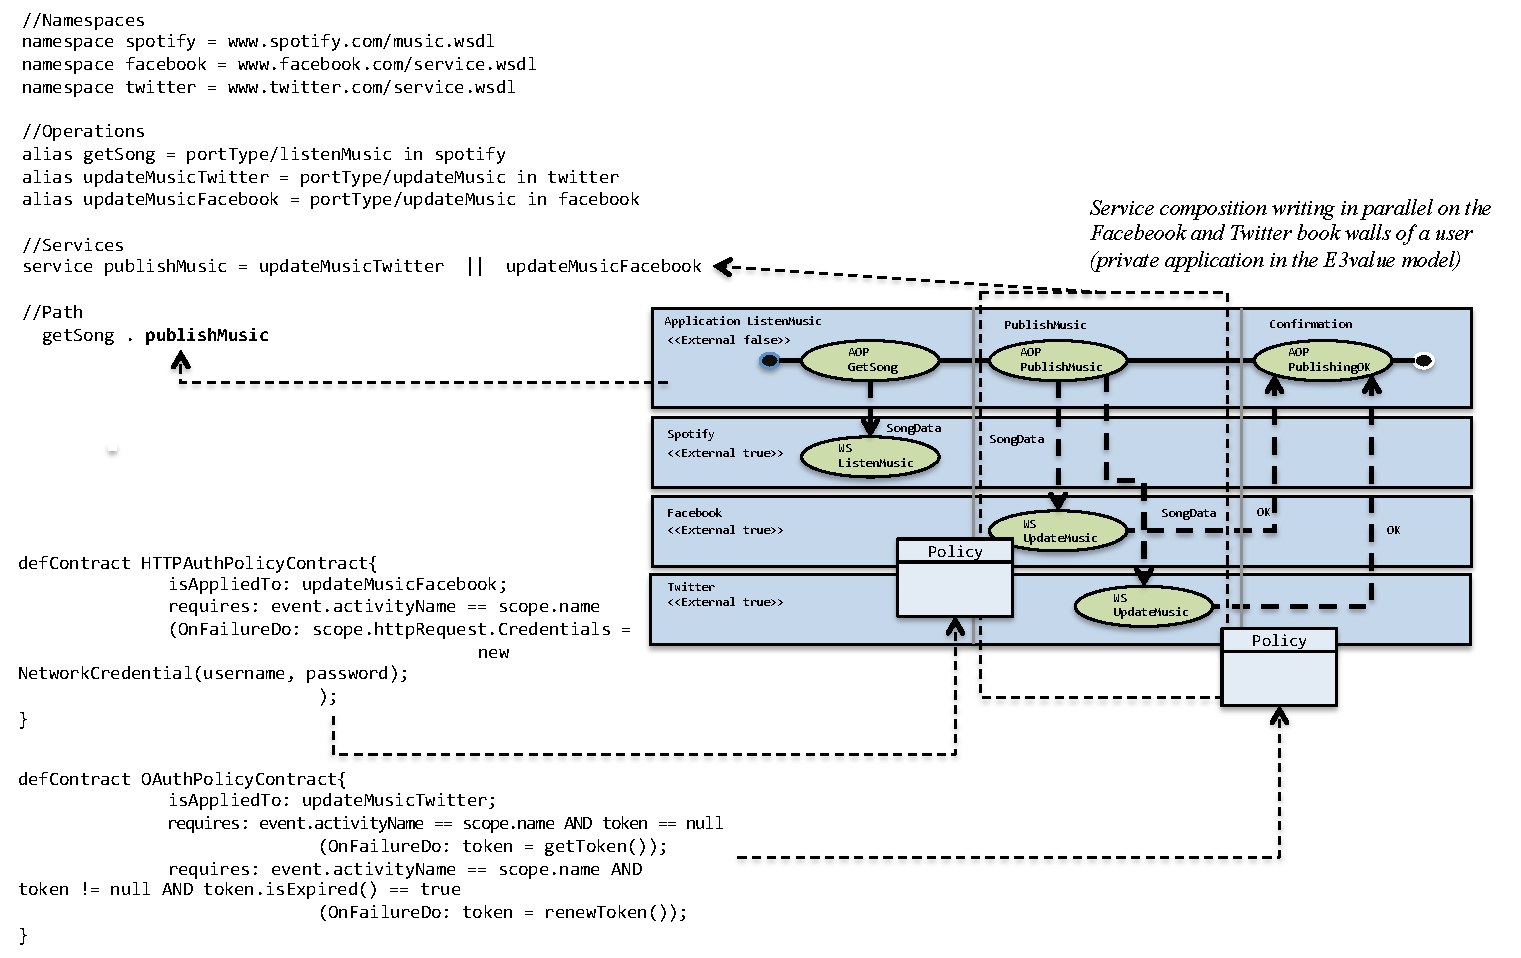
\includegraphics[width=0.85\textwidth]{figs/pews-expression}}
%\caption{Pews program implementing the "To Publish Music" application}
%\label{fig:pewsexpression}
%\end{figure}


%*********************************************************************************************************


%*********************************************************************************************************
\section{Implementation issues}\label{sec:implementation}

This section  describes the $\pi$-SOD-M development environment that implements the generation of {\em A-policies}' based services' compositions. For a given services' based application, the process  consists in generating the  code starting from a $\pi$-SCM modeling an application. Note that the services' composition model is not modeled from scratch, but it is the result of a general process defined by the $\pi$-SOD-M method in which a set of models are built following a service oriented approach \cite{decastro1}.

%We used the Eclipse Modeling Framework (EMF) to implement the whole model transformation process \footnote {The EMF project is a modeling framework and code generation facility for building tools and other applications based on a structured data model.}. From a model specification described in XMI, EMF provides tools and runtime support to produce a set of Java classes for the model, along with a set of adapter classes that enable viewing and command-based editing of the model, and a basic editor.
%In order to automate the transformation we specified  transformation rules using the ATL model transformation language Finally, in order to generate code we  used Acceleo \footnote{http://www.acceleo.org/pages/home/en}.

%..--..--..--..--..--..--..--..--..--..--..--..--..--..--..--..--..--..--..--..--..--..--..--..--..--..--..--..--..--..--..--..--..--..--..--..--..--..--
\subsection{$\pi$-SOD-M Development Environment}
%..--..--..--..--..--..--..--..--..--..--..--..--..--..--..--..--..--..--..--..--..--..--..--..--..--..--..--..--..--..--..--..--..--..--..--..--..--..--

Figure \ref{fig:policymanager} depicts a general architecture of the $\pi$-SOD-M Development Environment showing the set of plug-ins  developed in order to implement it. The environment implements the abstract architecture shown in Figure \ref{fig:sodm}. Thus, it consists of plug-ins implementing the $\pi$-SCM and $\pi$-{\sc Pews} meta-models used for defining models specifying services' compositions and their associated policies; and ATL rules for transforming  PSM models (model to model transformation) and finally generating code (model to text transformation).
\begin{figure}[htpb]
	\begin{center}
		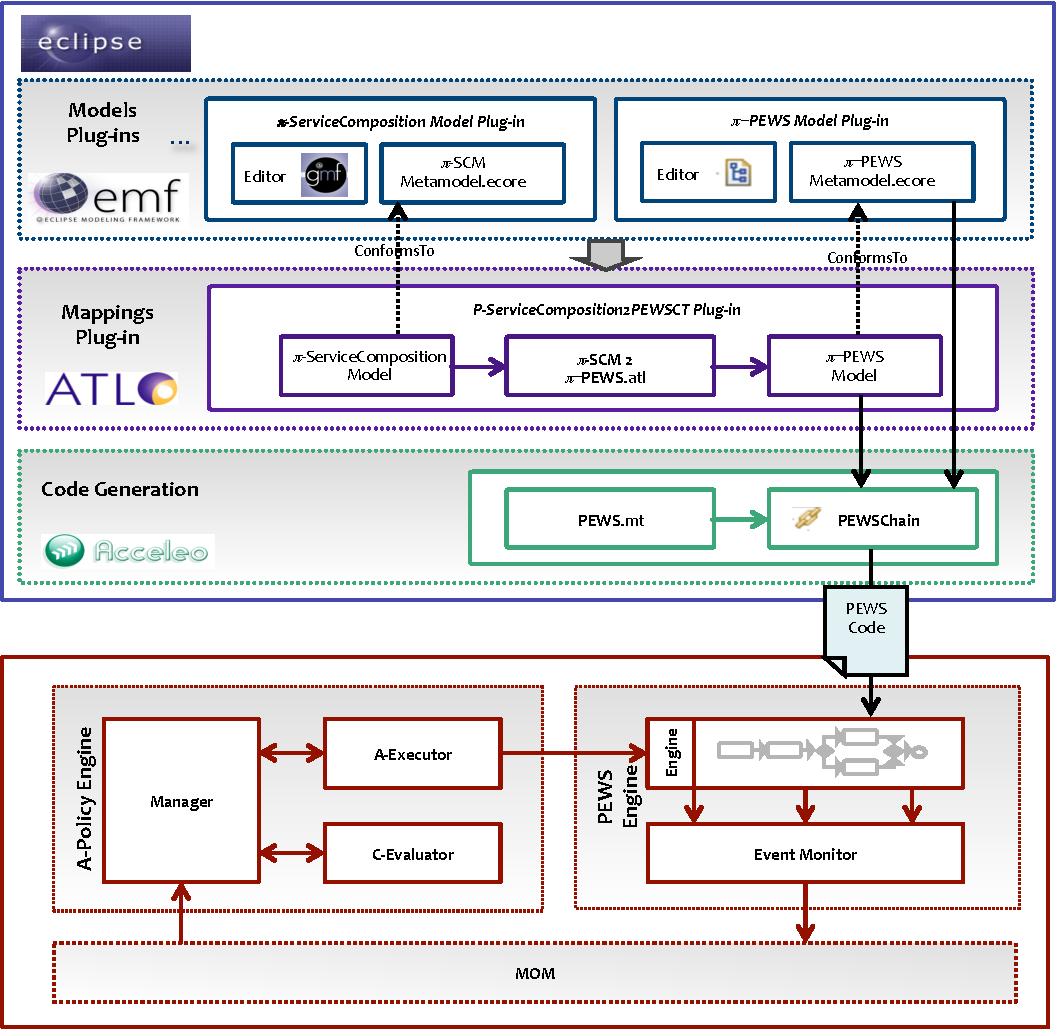
\includegraphics[width=0.60\textwidth]{figs/architecture}
	\end{center}
		\caption{$\pi$-SOD-M Development Environment}
   \label{fig:policymanager}
\end{figure}
\begin{itemize}
\item 	We  used the Eclipse Modeling Framework (EMF) \footnote {The EMF project is a modeling framework and code generation facility for building tools and other applications based on a structured data model.}   for implementing the meta-models  $\pi$- SCM and $\pi$-{\sc Pews}. Then, starting form these meta-models, we  developed the models' plug-ins needed to support the graphical representation of the $\pi$- SCM and $\pi$-{\sc Pews} models ($\pi$-ServiceCompostion Model and $\pi$-PEWS Model plug-ins).

\item	 We used  ATL \footnote{http://eclipse.org/atl/. An ATL program is basically a set of rules that define how source model elements are matched and navigated to create and initialize the elements of the target models.}
for  developing the mapping plug-in implementing the  mappings between models ($\pi$-ServiceComposition2$\pi$-PEWS Plug-in).

\item 	We  used Acceleo \footnote{http://www.acceleo.org/pages/home/en} for implementing  the code generation plug-in. We coded the pews.mt program  that implements the model to text transformation for generating executable code. It takes as input a $\pi$-PEWS model implementing a specific services' composition and it generates the code to be executed by the 
{\em A-policy} based services' composition execution environment. 

%\item Finally, we created a chain execution  to execute the model to text transformation.
\end{itemize}
%
%
%

%
As  shown in Figure \ref{fig:policymanager}, once an instance of a PEWS code is obtained starting form a particular $\pi$-services' composition model it can be executed over {\em A-policy} based services' composition execution environment  consisting of a composition engine and a {\em A-policy} manager.  The  {\em A-policy} manager  consists of three main components Manager, for scheduling the execution of rules, C-Evaluator and A-Executor respectively for evaluating rules' conditions and executing their actions. The {\em A-policy} Manager interacts with a composition engine thanks to a  message communication layer (MOM).


The composition engine manages the life cycle of the composition. Once a composition instance is activated, the engine schedules the composition activities according to the composition control flow.
Each activity is seen as the process where the service method call is executed.
The execution of an activity has four states: prepared, started, terminated, and failure.
The execution of the control flow (sequence, and/or split and join) can also be prepared, started, terminated and raise a failure.

At execution time, the evaluation of policies done by the {\em A-policy} manager must be synchronized with the execution of the services' composition (i.e., the execution of an activity or a control flow).  Policies associated to a scope are activated when the execution of its scope starts. A {\em A-policy} will have to be executed only if one or several of its rules is triggered. If several rules are triggered the {\em A-policy} manager first builds an execution plan that specifies the order in which such rules will be executed according to the strategies defined in the following section. 
%Once rules have been executed, the {\em A-policy} finishes its execution and returns to a sleeping state.
If rules belonging to several policies are triggered then policies are also ordered according to an execution plan. The execution of policies is out of the scope of this paper, the interested reader can refer to \cite{Espinosa-Oviedo2011a} for further details.
%The order of policies has implications on the global order of the rules to be executed.

%..--..--..--..--..--..--..--..--..--..--..--..--..--..--..--..--..--..--..--..--..--..--..--..--..--..--..--..--..--..--..--..--..--..--..--..--..--..--
\subsection{Validation}
%..--..--..--..--..--..--..--..--..--..--..--..--..--..--..--..--..--..--..--..--..--..--..--..--..--..--..--..--..--..--..--..--..--..--..--..--..--..--

We validated our approach  by implementing the "To Publish Music" application. It consists in atomically synchronizing  the status of a user's accounts according to the music she listens in Spotify and using authentication protocols for updating the walls' status in her Facebook and Twitter accounts.  Once the services' composition model has been annotated with the corresponding policies, then the reliable composition code can be generated using the rules defined for this purpose. Our implementation includes a  code generator that generates executable code for a reliable services' composition.
The model represents an services' composition expression and its associated policies. 


We tested the application  in order to see whether the coordination tolerated services unavailability keeping the status synchronized. Particularly, the token of the activity associated to Twitter was consistently obtained when the service was available. We also implemented a reference coordination without policies. We dealt with the availability exceptions by hand and the authentication protocols were embedded within the activities code. During our validation Twitter changed the authentication protocol and the maintenance of the application this implied re-programming the reference application. Instead, with the policies approach we only had to desactivate the corresponding policy and associate the appropriate one to the activity calling the service Twitter (one code line), and run the application again.


%*********************************************************************************************************

%*********************************************************************************************************
\section{Related works}\label{sec:related}

Related works to our approach include standards devoted for expressing non-functional constraints for services and services' compositions. They also include methods and approaches for modeling non-functional constraints.

%..--..--..--..--..--..--..--..--..--..--..--..--..--..--..--..--..--..--..--..--..--..--..--..--..--..--..--..--..--..--..--..--..--..--..--..--..--..--
%\noindent{\bf\em 
\subsection{Programming non-functional properties for services}
%..--..--..--..--..--..--..--..--..--..--..--..--..--..--..--..--..--..--..--..--..--..--..--..--..--..--..--..--..--..--..--..--..--..--..--..--..--..--
Current standards in services' composition implement functional, non-functional constraints and communication aspects by combining different languages and protocols. WSDL and SOAP among others are languages used respectively for describing services' interfaces and message exchange protocols for calling methods exported by such services. For adding a transactional behaviour to a services' composition it is necessary to implement WS-Coordination, WS-Transaction, WS-BussinessActivity and WS-AtomicTransaction. The selection of the adequate protocols for adding a specific non-functional constraints to a services' composition (e.g., security, transactional behaviour and adaptability) is responsibility of a programmer. As a consequence, the development of an application based on a services' composition is a complex and a time-consuming process. This is opposed to the philosophy of services that aims at facilitating the integration of distributed applications. Other works, like \cite{helga2}
introduce a model for transactional services composition based on
an advanced transactional model. \cite{samy} proposes an approach
that consists of a set of algorithms and rules to assist designers
to compose transactional services. In \cite{Vid04} the model
introduced in \cite{schuldt-etal-TODS} is extended to web services
for addressing atomicity.

%..--..--..--..--..--..--..--..--..--..--..--..--..--..--..--..--..--..--..--..--..--..--..--..--..--..--..--..--..--..--..--..--..--..--..--..--..--..--
%\noindent{\bf\em 
\subsection{Modeling non-functional properties}
%..--..--..--..--..--..--..--..--..--..--..--..--..--..--..--..--..--..--..--..--..--..--..--..--..--..--..--..--..--..--..--..--..--..--..--..--..--..--
There are few methodologies and approaches that address the explicit modeling  of non functional
properties for service based applications.   Software process methodologies for
building  services based applications have been proposed in\cite{PapazoglouH06,cdl2006,FeuerlichtM05,Ramollari_asurvey}, and they focus mainly on the modeling and construction process of services based business processes that represent the application logic of information systems.

 \textit{Design by Contract} \cite{HL05TACoS} is an approach for specifying web services and verifying them through runtime checkers before they are deployed. A contract adds behavioral information to a service specification, that is, it specifies the conditions in which methods exported by a service can be called. Contracts are expressed using the language \textit{jmlrac} \cite{LeavensCCRC02}.
 The \textit{Contract Definition Language} (CDL) \cite{cdl2006} is a XML-based
description language, for defining contracts for services. There are an associated architecture framework, design standards and a methodology, for developing applications using services.  A services' based application  specification is generated after several
 \cite{AbrialLNSS91} B-machines refinements that describe the services and their
compositions.
\cite{PapazoglouH06} proposes a methodology based on a SOA extension. This work defines a service
oriented business process development methodology with phases for business process development. The whole life-cycle is based on six phases: planning, analysis and design, construction and testing, provisioning, deployment, and execution and monitoring.
%IBM proposes a methodology for the development of SOA solutions, called SOMA \cite{soma}. SOMA defines a life-cycle with seven phases: business modeling and transformation, solution management, identification,
%specification, realization, implementation and deployment monitoring and management.

 %\cite{sommerville08} describes some key points for building services' based applications based on business process models that define the activities and information exchanged in a business processes. Activities in business process can be performed by services so that the model of business process
%represents a composition of services. It classifies services   as public utilities, business services or
%composition services. Software development that uses services involves creating programs for composing and configuring services to create new composite services. The service engineering process involves identifying services candidates, service interface and implementation definition, testing and deployment of each service.

%..--..--..--..--..--..--..--..--..--..--..--..--..--..--..--..--..--..--..--..--..--..--..--..--..--..--..--..--..--..--..--..--..--..--..--..--..--..--
%\noindent{\bf\em 
\subsection{Discussion}
%..--..--..--..--..--..--..--..--..--..--..--..--..--..--..--..--..--..--..--..--..--..--..--..--..--..--..--..--..--..--..--..--..--..--..--..--..--..--
As WS-*  and similar approaches, our work enables the specification and programing of  crosscutting aspects (i.e., atomicity, security, exception handling, persistence). In contrast to these approaches, our work specifies policies for a services' composition in an orthogonal way. Besides, these approaches suppose that non-functional requirements are implemented according a the knowledge that a programmer has of a specific application requirements but they are not derived in a methodological way, leading to ad-hoc solutions that can be difficult to reuse. In our approach, once defined {\em A-Policies} for a given application they can be reused and/or specialized for another one with the same requirements or that uses services that impose the same constraints. 

Furthermore, unlike methodologies and approaches providing best practices presented above, the main contribution of our proposal is that, integrated to a method that proposes meta-models at different levels (CIM, PIM and PSM) and extending the PSM meta-models, it enables  the design and development of services' based applications that can be reused and that are reliable. 

%*********************************************************************************************************

%*********************************************************************************************************
\section{Conclusions and future work}\label{sec:conclusions}
This paper presented $\pi$-SOD-M for specifying and designing reliable service based applications. We model and associate policies to  services' based applications that represent both systems' cross-cutting aspects and use constraints stemming from the services used for implementing them.  We extended the SOD-M method, particularly the $\pi$-SCM (services' composition meta-model) and $\pi$-{\sc Pews} meta-models for representing both the application logic and its associated non-functional constraints and then generating its executable code. We implemented the meta-models on the Eclipse platform and we validated the approach using a use case that uses authentication  policies.

Non-functional constraints are related to business rules associated to the general "semantics" of the application and in the case of services' based applications, they also concern the use constraints imposed by the services. We are currently working on the definition of a method for explicitly expressing such properties in the early stages of the specification of services based applications. Having such business rules expressed and then translated and associated to the services' composition can help to ensure that the resulting application is compliant to the user requirements and also to the characteristics of the services it uses.

Programming non-functional properties is not an easy task, so we are defining a set of predefined {\em A-policy} types with the associated use rules for guiding the programmer when she associates them to a concrete application. {\em A-policy} type  that can also serve as patterns for programming or specializing the way non-functional constraints are programmed.


%*********************************************************************************************************



%% The Appendices part is started with the command \appendix;
%% appendix sections are then done as normal sections
%% \appendix

%% \section{}
%% \label{}

%% References
%%
%% Following citation commands can be used in the body text:
%% Usage of \cite is as follows:
%%   \cite{key}          ==>>  [#]
%%   \cite[chap. 2]{key} ==>>  [#, chap. 2]
%%   \citet{key}         ==>>  Author [#]

%% References with bibTeX database:

\bibliographystyle{plain}
\bibliography{biblio}

%% Authors are advised to submit their bibtex database files. They are
%% requested to list a bibtex style file in the manuscript if they do
%% not want to use model1a-num-names.bst.

%% References without bibTeX database:

% \begin{thebibliography}{00}

%% \bibitem must have the following form:
%%   \bibitem{key}...
%%

% \bibitem{}

% \end{thebibliography}

\end{document}

%%
%% End of file `elsarticle-template-1a-num.tex'.
